% \usepackage{pgfplots}
% pgfplot settings
% \pgfplotsset{
% 			width=7cm,
% 			compat=newest, 
% 			label style={font=\small},
% 			legend style={font=\small},
% }

% command to create verical asymptotes
\providecommand{\vasymptote}[2][]{
    \draw [densely dashed,#1] ({rel axis cs:0,0} -| {axis cs:#2,0}) -- ({rel axis cs:0,1} -| {axis cs:#2,0});
}

% commands for setting color and lineweight of plots
\providecommand{\tangentcolor}{black}
\providecommand{\functioncolor}{black}
\providecommand{\tangentlineweight}{thick}
\providecommand{\functionlineweight}{ultra thick}

% plot image
 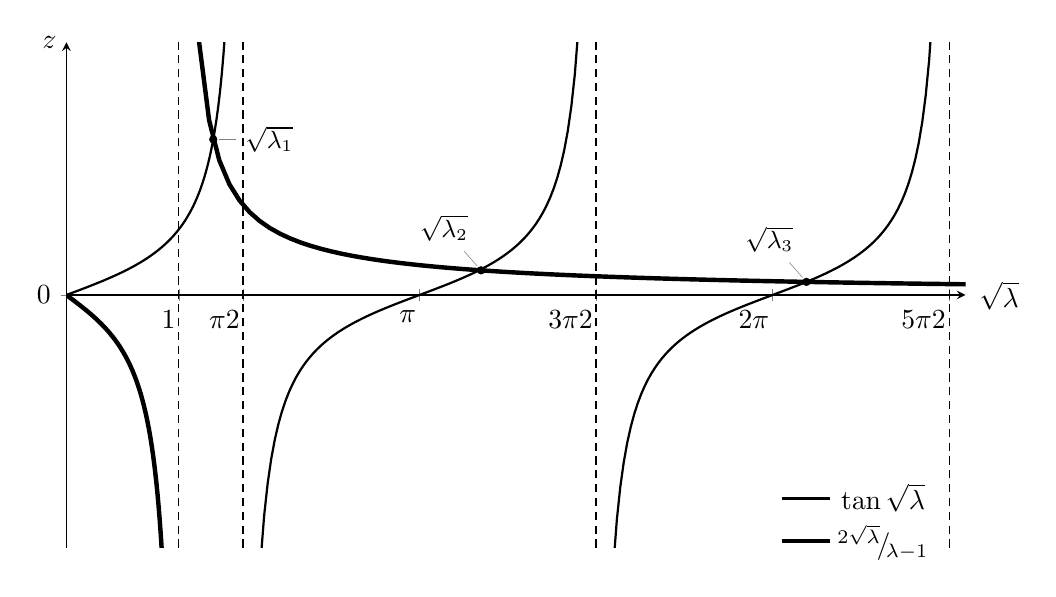
\begin{tikzpicture}
	\tikzset{dot/.style={fill=black,circle,scale=3}}  % node dot settings
	\begin{axis}[
		height=8cm,
		width=13cm,
		grid=none,
		axis x line=center,
		axis y line=left,
		ymin=-6,	ymax=6,
		xmin=0, 	xmax=8,		
		xlabel={$\sqrt{\lambda}$},
		ylabel={\rotatebox{90}{$z$}},
		x label style={at={(1.07,0.45)}},
		y label style={at={(0,0.999)}},
		xtick={0,1,1.5708,3.14159,4.7123889,6.283185307,7.853981634},
		xticklabels={$0$, $1$, $\Frac{\pi}{2}$, $\pi$, $\Frac{3\pi}{2}$, $2\pi$, $\Frac{5\pi}{2}$},
		xticklabel style={inner xsep=1pt,anchor=north east},
		ytick={0},
		legend style={draw=none,at={(0.975,0.15)}},
		]
		% tan(s)
		\addplot[\tangentlineweight,domain=0:(pi/2),samples=101,unbounded coords=jump,color=\tangentcolor,mark=none]{tan(deg(x))};
		% f(s)
		\addplot[\functionlineweight,domain=0:1,samples=101,unbounded coords=jump,color=\functioncolor,mark=none]{(2*x)/(x^2-1)};
		\addplot[\functionlineweight,domain=1:10,samples=101,unbounded coords=jump,color=\functioncolor,mark=none]{(2*x)/(x^2-1)};
		% Legend Entries
		\addlegendentry{$\tan\sqrt{\lambda}$}
	    \addlegendentry{$ ^{2\sqrt{\lambda}}\! /\! _{\lambda-1} $} %\frac{2\sqrt{\lambda}}{\lambda-1}
		% Remaining portions of tan(s)
		\addplot[\tangentlineweight,domain=(pi/2):(3*pi/2),samples=101,unbounded coords=jump,color=\tangentcolor,mark=none]{tan(deg(x))};
		\addplot[\tangentlineweight,domain=(3*pi/2):7.8,samples=101,unbounded coords=jump,color=\tangentcolor,mark=none]{tan(deg(x))};
		% Vertical asymptotes
		\vasymptote{1}
		\vasymptote{1.570796327}
	   	\vasymptote{4.71238898}
		\vasymptote{7.853981634}
		% Nodes for lambda_i
		\node at (axis cs:1.30654,3.6957) [dot,pin={[pin distance=6pt]0:\small{$\sqrt{\lambda_1}$}},inner sep=0pt] {};
		\node at (axis cs:3.68900,.585526) [dot,pin={[pin distance=5pt]100:\small{$\sqrt{\lambda_2}$}},inner sep=0pt]{};
		\node at (axis cs:6.58462,0.3109) [dot,pin={[pin distance=5pt]100:\small{$\sqrt{\lambda_3}$}},inner sep=0pt]{};	
    \end{axis}
\end{tikzpicture}